
\section{Assumptions and Notations}

\subsection{Assumptions and Justifications}

To simplify problem, make it convenient to construct simulation model and ensure it's effectiveness, following basic assumptions are made, each of which is properly justified.

\begin{itemize}
\item {\bf Data Preprocess and Country Mapping}. 

Data is cleaned and preprocessed to make it more suitable. We set the ice sports aside, combine various teams of one country, and map the countries which no longer exist to the current existing country. It's a rather difficult task since countries have changed a lot during the past century, but it's necessary to stick to the current world map.

\item {\bf Relationship between Medal counts and Historical data}. 

Most data provided is examined to be accurate and reliable, although some may not be the same as the data provided from other sources. Few of the data is examined and changed since it's too faraway from reality. Medal counts are also assumed to be related to multiple variables:years, gender, athletes and number of sports, diciplines, events,etc.

\item {\bf Countries that will possibly take part in the 2028 Olympics}. 

Countries that have taken part in 2024 Olympics will also take part in 2028 Olympics. There's no reason for them not to attend the Olympics, and it's impossible to estimate medal of new countries if they've never taken part in the Olympics using historical data. Russia is also assumed to participate in the 2028 Olympics, whether the athletes will be able to compete under the Russian flag or not, their country is called Russia. 

\item {\bf Possible Sports in 2028}. 

There's said to be five new sports in the 2028 Olympics, but we set them aside because we don't have enough data to predict the medal counts of these events. Similarly, we set aside the sports that will be removed from the Olympics in 2028, and assume that most sports are like that in 2024 or their most common appearance in history(Such as gymnastics).


\end{itemize}

Other details will be stated in the following sections when we discuss the specific models.

\subsection{Notations}

\begin{center}
\begin{tabular}{clcl}
{\bf Symbols} & {\bf Definitions} & {\bf Symbols} & \quad {\bf Definitions} \\[0.25cm]
$N_u$ & Number of no medal countries & $\text{I}_{f}$ &  Feature Importance \\[0.2cm]
$\text{P}_{total}$ & Total Key Event index of a country & $\text{I}_{m}(s,j)$ & Impurity for split $s$ on feature $j$ \\[0.2cm]
$\text{M}_{ei}$ & Medal counts of event $i$ & $h_k(\mathbf{x})$ & Leaf value of multiple features $x$\\[0.2cm]
$\text{M}_{tc}$ & Total number of medals for country & $\alpha_k$ & Weight for leaf value $k$ \\[0.2cm]
$\text{X}_{c}$ & Centered variables using PCA & $L(\theta)$ & Legendary Index \\[0.2cm]
\end{tabular}
\end{center}
\noindent Define the Main Parameters. Other Specific Notations will be listed and explained later.

\section{Data Preprocessing}
\subsection{Data Cleaning}
\begin{itemize}
    \item \textbf{Garbled Code}
\end{itemize}

\begin{figure}[h]
    \centering
    \begin{minipage}{0.8\textwidth}
        \centering
        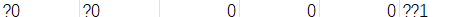
\includegraphics[width=\textwidth]{../figures/bad_1.png}
        \caption{bad data}
        \label{fig:bad_1}
    \end{minipage}\hfill
    \begin{minipage}{0.2\textwidth}
        \centering
        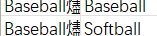
\includegraphics[width=\textwidth]{../figures/bad_2.png}
        \caption{bad text}
        \label{fig:bad_2}
    \end{minipage}
\end{figure}

We carefully examine the data and find that there are some garbled codes in the data, which may be caused by the encoding of the data. They are replaced by the correct text.

\begin{itemize}
    \item \textbf{Null, Duplicated Values and Renaming}
\end{itemize}

\begin{lstlisting}[caption=Data Cleaning]
data.fillna(0, inplace=True)
data.drop_duplicates(inplace=True)
athletes.rename(columns={'Team': 'Country'}, inplace=True)
\end{lstlisting}

Team are renamed to Country in the athletes data so that there won't be Germany-1.

\begin{itemize}
    \item \textbf{Data Splitting}
\end{itemize}

\begin{lstlisting}[caption=Data Splitting]
    data.fillna(0, inplace=True)
    data.drop_duplicates(inplace=True)
    athletes.rename(columns={'Team': 'Country'}, inplace=True)
    \end{lstlisting}

    \begin{itemize}
        \item \textbf{Remove unnecessary data}
    \end{itemize}
\begin{lstlisting}[caption=Remove Ice Sports]
    ice_sports = ['Figure Skating', 'Ice Hockey']
    programs = programs[~programs['Sport'].isin(ice_sports)]
    athletes = athletes[~athletes['Sport'].isin(ice_sports)]
\end{lstlisting}

\begin{lstlisting}[caption=Remove Program from 1906]
# Remove program from the year 1906
program = program[program['Year'] != 1906]    
\end{lstlisting}

\subsection{Country Mapping}

\begin{lstlisting}[caption=Country Mapping]
country_mapping = {# map due to the change of country in history
    'Soviet Union': 'Russia','Unified Team': 'Russia',
    'West Germany': 'Germany','East Germany': 'Germany',
    'Yugoslavia': 'Serbia',
    'Bohemia': 'Czech Republic','Czechoslovakia': 'Czech Republic',
    'Virgin Islands': 'United States',
}
# NOC mapping is similar.Only part of the country_mapping is shown here.There're also map between NOC and country.
athletes['NOC'] = athletes['NOC'].replace(noc_mapping)
medals['NOC'] = medals['NOC'].replace(country_mapping)
\end{lstlisting}

\subsection*{Primary processed data: The `Top 10s'}

\begin{figure}[h]
    \centering
    \begin{minipage}{0.4\textwidth}
        \centering
        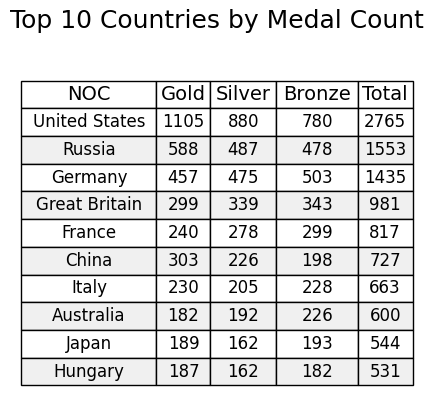
\includegraphics[width=\textwidth]{../figures/top_10_countries.png}
        \caption{top $10$ countries}
        \label{fig:top_10_countries}
    \end{minipage}\hfill
    \begin{minipage}{0.4\textwidth}
        \centering
        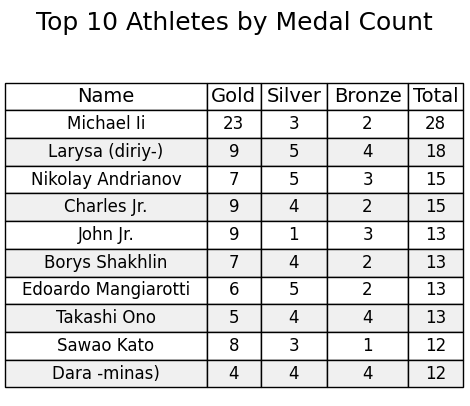
\includegraphics[width=\textwidth]{../figures/top_10_athletes.png}
        \caption{top $10$ athletes}
        \label{fig:top_10_athletes}
    \end{minipage}
\end{figure}